% Tutorial 2
%
% @author Jonathan Karr, jkarr@stanford.edu
% @affiliation Covert Lab, Department of Bioengineering, Stanford University
% @lastupdated 4/5/2009
\documentclass[mathserif]{beamer}

%%%%%%%%%%%%%%%%%%%%%%%%%%%%%%%%%%%%%%%%%%%%%%%%%%
%%% Style                                      %%%
%%%%%%%%%%%%%%%%%%%%%%%%%%%%%%%%%%%%%%%%%%%%%%%%%%
\mode<presentation>{
  \usetheme{tutorial}}


%%%%%%%%%%%%%%%%%%%%%%%%%%%%%%%%%%%%%%%%%%%%%%%%%%
%%% Title                                      %%%
%%%%%%%%%%%%%%%%%%%%%%%%%%%%%%%%%%%%%%%%%%%%%%%%%%

\title[NetworkPainter Tutorial \#2]{NetworkPainter Tutorial \#2\\Visualizing Experimental Data}
\author[Jonathan Karr]{Jonathan R. Karr\\jkarr@stanford.edu}
\institute[Stanford University]{
  Department of Bioengineering\\
  Stanford University}
\subject{Systems Biology}
\date[]{}

\begin{document}

\begin{frame}
  \titlepage
\end{frame}

%%%%%%%%%%%%%%%%%%%%%%%%%%%%%%%%%%%%%
%%% teaser
%%%%%%%%%%%%%%%%%%%%%%%%%%%%%%%%%%%%%
\begin{frame}
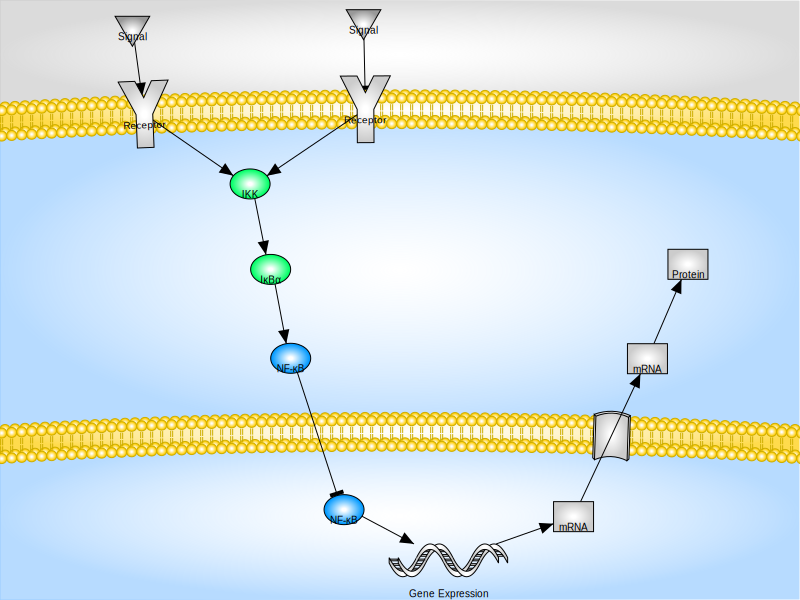
\includegraphics[width=\textwidth]{NF-kB.pdf}
\end{frame}

\begin{frame}
\includemovie[autoplay,mouse=false]{\textwidth}{\textheight}{NF-kB.swf}
\end{frame}

%%%%%%%%%%%%%%%%%%%%%%%%%%%%%%%%%%%%%
%%% outline
%%%%%%%%%%%%%%%%%%%%%%%%%%%%%%%%%%%%%
\begin{frame}
\vskip-.2in
\begin{columns}[t]
\begin{column}{2.1in}

\begin{block}<1->{\small Tutorial \#1\\Creating Network Models}
\scriptsize
\begin{itemize}
\item Register a NetworkPainter user account
\item Create an NF-$\kappa$B network model
\item Export images of the NF-$\kappa$B network
\item Save the network to the NetworkPainter database
\end{itemize}
\end{block}
\vskip.1in

\begin{block}<2->{\small Tutorial \#2\\Visualizing Experimental Data}
\scriptsize
\begin{itemize}
\item Open the saved NF-$\kappa$B network
\item Associate the network with experimental data from CytoBank
\item Export animations of the NF-$\kappa$B network
\end{itemize}
\end{block}

\end{column}
\begin{column}{.05in}

\end{column}
\begin{column}{2.1in}

\begin{block}<3->{\small Tutorial \#3\\Advanced Topics}
\scriptsize
\begin{itemize}
\item Automatic network layout
\item Advanced rendering options
\item Collaboration: sharing \& publishing networks
\end{itemize}
\end{block}

\end{column}
\end{columns}
\end{frame}

%%%%%%%%%%%%%%%%%%%%%%%%%%%%%%%%%%%%%
%%% tutorial
%%%%%%%%%%%%%%%%%%%%%%%%%%%%%%%%%%%%%
\begin{frame}{Outline}
\begin{itemize}
\item Login to NetworkPainter
\item Open NF-$\kappa$B network
\item Open Experiment Manager
\item Associate network with experimental data
\item View animation
\item Explore heatmaps
\item Logout
\end{itemize}
\end{frame}

%%%%%%%%%%%%%%%%%%%%%%%%%%%%%%%%%%%%%
%%% summary
%%%%%%%%%%%%%%%%%%%%%%%%%%%%%%%%%%%%%
\begin{frame}
\begin{columns}
\begin{column}{3.5in}
\begin{center}
\begin{beamercolorbox}[rounded=true,shadow=true,center,sep=0.01cm]{structure2}
\LARGE
Summary
\end{beamercolorbox}
\begin{itemize}
\item Opened the saved NF-$\kappa$B network
\item Associated the network with experimental data from CytoBank
\item Exported animations of the NF-$\kappa$B network
\end{itemize}
\end{center}
\end{column}
\end{columns}
\end{frame}

\begin{frame}
\begin{columns}
\begin{column}{3.5in}
\begin{center}
\begin{beamercolorbox}[rounded=true,shadow=true,center,sep=0.01cm]{structure2}
\LARGE
Next Time
\end{beamercolorbox}
\begin{itemize}
\item Automatic network layout
\item Advanced rendering options
\item Collaboration: sharing \& publishing networks
\end{itemize}
\end{center}
\end{column}
\end{columns}
\end{frame}

%%%%%%%%%%%%%%%%%%%%%%%%%%%%%%%%%%%%%
%%% questions
%%%%%%%%%%%%%%%%%%%%%%%%%%%%%%%%%%%%%
\begin{frame}{}
\begin{columns}
\begin{column}{3.5in}
\begin{center}
\begin{beamercolorbox}[rounded=true,shadow=true,center,sep=0.01cm]{structure2}
\LARGE
Questions
\end{beamercolorbox}
\vskip.1in
\large
covertlab.stanford.edu/projects/NetworkPainter\\
\vskip.05in
NetworkPainter@lists.stanford.edu
\end{center}
\end{column}
\end{columns}
\end{frame}

\end{document}
